\section{Ownership Assignment}
\label{section:ownership}

The results section discusses the empirical analysis of the clustering methods tested during the implementation of the Ownership Assignment process. 

\subsection{Dataset}
The experiment design is simple and designed to provide an upper bound for performance on an optimal dataset with no noise (the Swan Valley wineries dataset.) 
The Swan Valley Wineries dataset consists of 31 wineries retrieved from OSM and \~150 objects hand-labeled across 6 of those 31 locations with ground-truth location labels.


\subsection{Method}
Using 1/distance to nearest location as probability of assigning an object to that location.
Achieves a fuzzy clustering of objects to locations, since objects can be assigned to multiple locations with some probability p.


\subsection{Results}
Examining the errors reveals the following insights about each clustering technique. 

\textbf{When K-Means clusters incorrectly, labels are still correct.} When $K$ exceeds the number of clusters, it fragments the actual clusters. 
However, in ideal conditions like the Wineries Dataset, where locations are separated, the centroids of these cluster fragments are still closest to the correct location. 
As a consequence, they are correctly labeled despite being incorrectly clustered. We expect the accuracy will drop when locations are more densely packed. However, when we aim to process all objects and locations in a region concurrently, the number of clusters will likely approach the number of locations, and the issue will be less pronounced. 


RESULTS TABLE HERE.........
\begin{table}[h!]
	\begin{center}
		\begin{tabular}{ |c|c|c|c| } 
			\hline
			Location & Precision & Recall \\
			\hline
			\multirow{7}{4em}{K-Means} 
                & $K=1$ & 1 \\ 
			& $K=6$ & 6  \\ 
			& $K=31$ & 31 \\ 
                & $K=1$ & 1 \\ 
			& $K=6$ & 6  \\ 
			& $K=31$ & 31 \\ 
   			& $K=31$ & 31 \\ 
			\hline
		\end{tabular}
		\label{table:clustering}
		\caption{..............}
	\end{center}
\end{table}


\begin{figure*}[ht]
\label{fig:cmeans}        
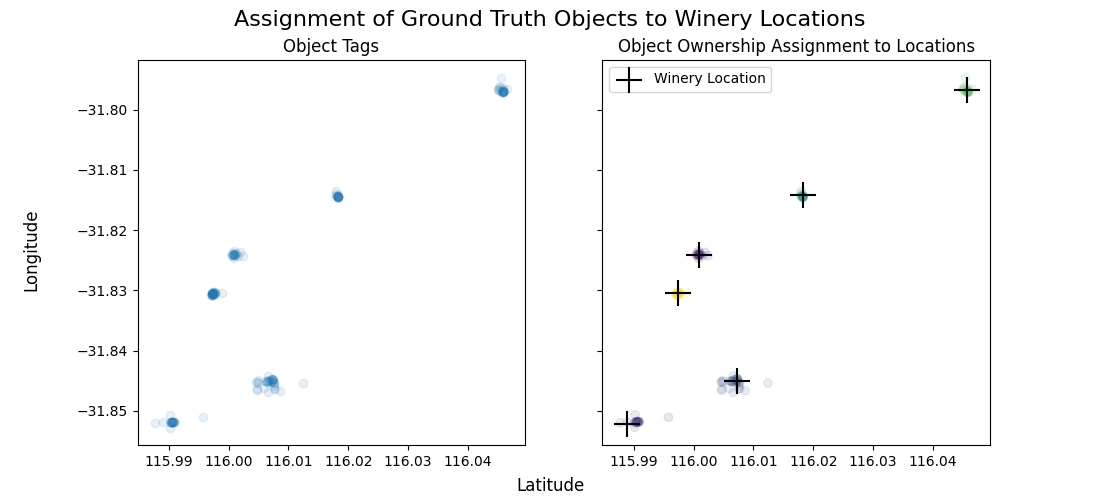
\includegraphics[width=\textwidth]{papers/figures/gestalt_cmeans.png}
\centering
\caption[width=\textwidth]{............}
\end{figure*}



\subsection{OLD, INTEGRATE OR DELETE........}
Ownership assignment is implemented in Python in two ways. The first is the trivial implementation, where the location returned from the OSM query is a bounding polygon. 
In this case, if the point lies within the minimal enclosing rectangle of the polygon, it is added as a 'member' of that location. 
The second, more common (and more challenging approach) formulates an unsupervised learning problem using clustering libraries from \textit{scikit-learn}\footnote{\href{https://pypi.org/project/scikit-learn/}{Scikit-Learn PyPI Repo}}. 
Given a collection of objects and a collection of locations within a bounding box region, clustering assigns each object to its 'parent' location. 
Under the assumption that the number of locations equals the number of clusters, K-Means clustering proved to be the most effective approach. 
After clustering the objects, we determine the centroid of the object cluster. Given a KD tree constructed from location point coordinates, a nearest neighbor search on the KD tree with a query parameter of the object centroid yields the nearest location and is assigned ownership of that cluster
A detailed performance comparison is in section \ref{section:results}. 

Overall, initial proof-of-concept clustering uses K-Means and DBSCAN clustering. An optimal solution to the ownership assignment problem is an exciting and unusual clustering problem. 
Assuming that the collection of locations is complete and that the point coordinate of the location is central to the collection of objects that belong to that location, the clustering problem is the assignment of an arbitrary number of objects to any of a set of possible centroids. Not every centroid will have objects, and objects are not uniformly distributed. Initial investigation into the DVBSCAN algorithm Ram et al. proposed in 2010 presents a promising direction to resolve this problem.\cite{Ram2010} 

Overall, the Ownership Assignment process needs to produce a data structure that will permit set membership checking for search and set the conditions for the concept mapping process. It is the most complete component of \textit{GESTALT}. The choice of clustering algorithm needs refinement, and location-based bloom filters need to be implemented to support efficient search, but it is otherwise functional. 